\section[Bezpečnost výzkumných reaktorů]{Bezpečnostní aspekty provozu výzkumných reaktorů}

\subsection{Úvod do bezpečnosti jaderných reaktorů (obecně)}

Skutečnost, že reaktor existuje, neznamená, že je automaticky bezpečný, a provoz reaktoru neznamená automaticky jeho bezpečný provoz. Klíčové otázky, které je třeba si klást, zahrnují:

\begin{itemize}
    \item Co je bezpečné? Co je nebezpečné? Co je dostatečně bezpečné?
    \item Kdo může deklarovat, že je něco bezpečné (nebo nebezpečné)?
    \item Jak můžeme měřit bezpečnost?
    \item Máme stejné standardy nebo limity pro bezpečnost na celém světě?
\end{itemize}

\subsubsection*{PROČ? -- 3S koncept}

Každý reaktor musí splňovat koncept 3S:

\begin{itemize}
    \item \textbf{Safety (bezpečnost)}
    \item \textbf{Security (ochrana)}
    \item \textbf{Safeguard (zárukový proces)}
\end{itemize}

Bezpečný a bezpečně chráněný provoz jakékoliv jaderné instalace je dosažen prostřednictvím plného přijetí, dodržování a ověřování všech požadavků na bezpečnost, ochranu a záruky.

\subsubsection*{KDY? -- Životní cyklus reaktoru}

Bezpečnostní požadavky se týkají celého životního cyklu reaktoru, který zahrnuje:

\begin{itemize}
    \item Záměr stavby jaderné instalace
    \item Výběr lokality a hodnocení místa
    \item Návrh
    \item Výstavba
    \item Uvádění do provozu
    \item Provoz
    \item Vyřazování z provozu
    \item Uvolnění z regulačního dohledu
\end{itemize}

\subsubsection*{KDO? -- Klíčové subjekty reaktoru}

V oblasti jakékoli jaderné instalace (například výzkumný reaktor nebo jaderná elektrárna) působí tři hlavní subjekty:

\begin{itemize}
    \item Stát
    \item Regulační orgán
    \item Provozovatel
\end{itemize}

Mezinárodní agentura pro atomovou energii (IAEA) hraje také významnou roli.

\subsubsection*{JAK? - Základní principy bezpečnosti reaktoru}

Bezpečnost reaktoru je velmi složitý úkol, který by měl být řešen prostřednictvím úzké spolupráce mezi všemi klíčovými subjekty (stát, regulační orgán a provozovatel). Tento proces by měl být iterativní a periodický.

Filozofie bezpečnosti reaktoru zahrnuje bezpečnostní cíle založené na konceptu víceúrovňové obrany (\textit{defence in depth}) a bezpečnostních principech. Příklad víceúrovňové obrany zahrnuje bariéry, které chrání proti úniku štěpných produktů do prostředí:

\begin{itemize}
    \item Bariéra 1: Materiál jaderného paliva (matrice)
    \item Bariéra 2: Pokrytí jaderného paliva
    \item Bariéra 3: Primární okruh
    \item Bariéra 4: Ochranná obálka (containment)
\end{itemize}

\begin{figure}[H]
    \centering
    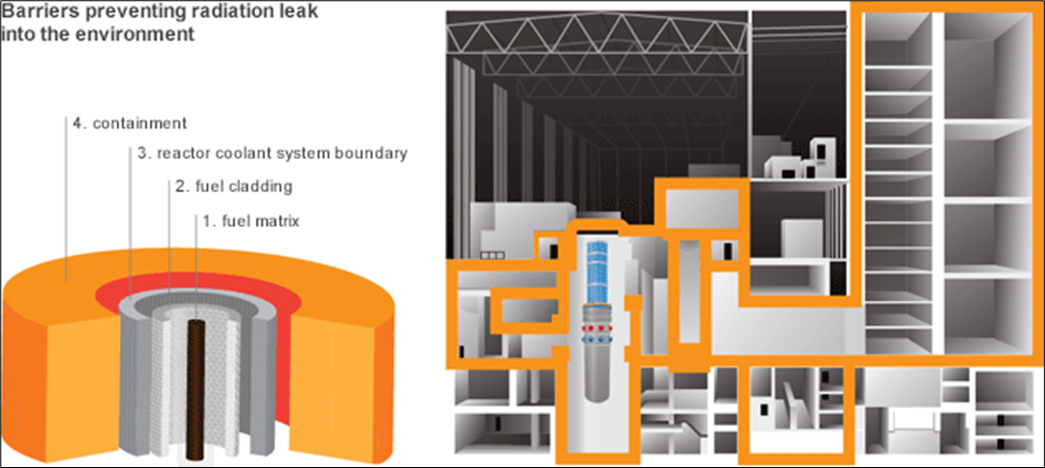
\includegraphics[width=0.75\linewidth]{img/DID.png}
    \caption{Ochrana do hloubky.}
    \label{fig:enter-label}
\end{figure}

Lze rozeznávat 5 úrovní ochrany do hloubky:

\begin{enumerate}
    \item Prevence abnormálního provozu a poruch
    \item Řízení abnormálního provozu a detekce poruch
    \item Řízení havárií v rámci návrhové základny
    \item Řízení těžkých podmínek zařízení, prevence eskalace havárie a zmírnění následků těžkých havárií
    \item Zmírnění radiologických důsledků významného úniku radioaktivních látek
\end{enumerate}

S tím souvisí nějaké technické a administrativní požadavky, zahrnující:

\begin{itemize}
    \item Redundance: Použití tří stejných měřicích linek systému I\&C reaktoru.
    \item Diverzita: Použití různých typů detektorů nebo softwaru pro stejné měřicí linky.
    \item Nezávislost: Například systémy odstavení reaktoru využívající spouštění tyčí a odvodnění bazénu.
    \item Konzervativnost: Vždy předpokládat nejhorší možné scénáře.
    \item Kvalita technologií a procesů: Zajištění kvality.
    \item Vysoká úroveň výcviku klíčového personálu ve všech fázích životního cyklu reaktoru.
\end{itemize}

Otázky "Co je bezpečné? Co je nebezpečné? Co je dostatečně bezpečné?" jsou klíčové pro hodnocení bezpečnosti jaderných zařízení. Bezpečnostní analýza zahrnuje celkový rozsah fyzikálně dosažitelných hodnot zkoumaného parametru, který je analyzován, aby byl určen bezpečný rozsah tohoto parametru. Tyto analýzy jsou podrobně popsány v dokumentu \textit{Bezpečnostní analýza} (Safety Analysis Report, SAR).

Omezení zkoumaného parametru jsou dále definována včetně bezpečnostních rezerv, které zajišťují ochranu i za neobvyklých okolností. Tato omezení a bezpečnostní rezervy jsou popsány v dokumentu \textit{Provozní limity a podmínky} (Operational Limits and Conditions, OLC).

\subsection{Bezpečnost výzkumných reaktorů}

Bezpečnost výzkumných reaktorů zahrnuje specifické aspekty související s jejich provozem. Výzkumné reaktory jsou citlivější na nehody související s kritičností kvůli zpoždění negativní zpětné vazby při nízkých úrovních výkonu (řádově watty až kilowatty). Časté změny výkonu a reaktivity vyžadují zvýšenou pozornost kinetice a dynamice reaktoru. Další důležitou roli hraje vliv experimentálního vybavení a vzorků umístěných v jádru nebo reflektoru, které mohou významně ovlivnit provoz reaktoru.

Hlavní faktory ovlivňující bezpečnost výzkumných reaktorů:

\begin{itemize}
    \item Využití reaktoru
    \item Experimentální vybavení
    \item Modifikace technologie reaktoru, I\&C a experimentálních zařízení
    \item Odstupňovaný přístup
    \item Prodloužené odstávky
\end{itemize}

\textbf{Postulované iniciační události (PIE):}

Pro výzkumné reaktory byly identifikovány různé postulované iniciační události, které mohou vést k nehodám:

\begin{itemize}
    \item \textbf{Ztráta elektrického napájení}
    \item \textbf{Nadměrná vnesená reaktivita:}
    \begin{itemize}
    \item Kritičnost během manipulace s palivem a jeho zavádění
    \item Selhání pohonu nebo celého systému pohonu regulačních tyčí
    \item Zavedení studené nebo horké vody
    \item Změny v moderátoru (například tvorba bublin, únik těžké vody \textit{D\textsubscript{2}O} do systému s lehkou vodou \textit{H\textsubscript{2}O})
    \item Vliv experimentů a experimentálních zařízení (například zaplavení, tvorba dutin, teplotní vlivy, zavedení štěpného materiálu nebo odstranění absorpčního materiálu)
    \item Neúmyslné vysunutí regulačních tyčí
    \item Chyby při údržbě zařízení pro řízení reaktivity
    \item Falešné signály z řídicího systému
\end{itemize}
    \item \textbf{Ztráta toku chladicí kapaliny}
    \begin{itemize}
    \item Selhání primárního čerpadla
    \item Snížení průtoku primární chladicí kapaliny (např. kvůli selhání ventilu nebo blokaci v potrubí či tepelném výměníku)
    \item Blokace kanálu pro palivo nebo snížení průtoku (např. kvůli cizímu materiálu)
\end{itemize}
    \item \textbf{Ztráta chladicí kapaliny}
    \begin{itemize}
        \item prasknutí potrubí nebo poškození bazénu
    \end{itemize}
    \item \textbf{Chybné zacházení s vybavením nebo jeho selhání}
    \item \textbf{Speciální interní události}
    \begin{itemize}
        \item například požáry, výbuchy, interní záplavy nebo bezpečnostní incidenty
    \end{itemize}
    \item \textbf{Externí události}, jako jsou zemětřesení, záplavy, tornáda nebo požáry
    \item \textbf{Lidské chyby}
\end{itemize}

Bezpečnost výzkumných reaktorů je zajištěna konceptem obrany do hloubky, který zahrnuje následující 3 úrovně (poslední 2 nejsou pro výzkumné reaktory):

\begin{enumerate}
    \item Prevence abnormálního provozu a selhání
    \item Řízení abnormálního provozu a detekce selhání
    \item Řízení nehod v rámci návrhových podmínek
    \item \textcolor{red}{Řízení těžkých podmínek v elektrárně a zmírnění následků vážných nehod}
    \item \textcolor{red}{Zmírnění radiologických důsledků významného uvolnění radioaktivního materiálu}
\end{enumerate}

\textbf{Bezpečnostní zpráva (SAR):}

Bezpečnostní zpráva pro výzkumné reaktory (Safety analysis report (SAR)) má strukturu přizpůsobenou specifickým potřebám těchto zařízení, přestože obsah je obdobný jako u energetických reaktorů. Obsahuje následující kapitoly:

\begin{itemize}
    \item Popis zařízení
    \item Bezpečnostní cíle a inženýrské požadavky
    \item Charakteristika lokality
    \item Budovy a konstrukce
    \item Chladicí systémy a další propojené systémy
    \item Bezpečnostní systémy, instrumentace a kontrola
    \item Limity provozu a podmínky
    \item Plánování a připravenost na mimořádné situace
\end{itemize}

\textbf{Limity a podmínky (LaP):}

Na základě \textit{Operational Limits and Conditions and Operating Procedures for Research Reactors}, IAEA Specific Safety Guide, NS-G-4.4, IAEA 2008 a IAEA Specific Safety Guide, SSG-20, IAEA 2012:

\begin{itemize}
    \item Bezpečnostní limity
    \item Nastavení bezpečnostních systémů
    \item Omezující podmínky pro bezpečný provoz
    \item Požadavky na dohled
    \item Administrativní požadavky
\end{itemize}

\subsection{Nehody na výzkumných reaktorech}

Specifické aspekty jaderné bezpečnosti na výzkumných reaktorech vyplývají z jejich citlivosti na nehody související s kritičností. Tato citlivost je způsobena zpožděním negativních zpětných vazeb při nízkém výkonu (řádově watty až kilowatty). Časté změny výkonu a reaktivity vyžadují zvýšenou pozornost kinetice a dynamice reaktoru. Navíc experimentální instrumentace a vzorky v jádru a reflektoru mohou významně ovlivnit provoz reaktoru.

Typickými nehodami jsou nehody s kritičností, nehody při přechodových stavech, ozáření personálu.

\begin{itemize}
    \item Kritičnostní nehody, například:
        \begin{itemize}
            \item Skládání AZ
            \item Zavážení paliva
            \item Přesun paliva
            \item Úpravy jádra
            \item Manipulace s reflektorem nebo absorpčními materiály
            \item Experimentální instrumentace (vkládání, odstraňování, selhání)
            \item Lidské chyby
        \end{itemize}
    \item Přechodové nehody (transientní nehody)
    \item Radiační expozice personálu reaktoru
\end{itemize}

\subsubsection{Příklad nehody s kritičností -- RA-2}

Dne 23. září 1983 došlo k vážné nehodě v argentinském výzkumném reaktoru RA-2, umístěném v Centru Atómico Constituyentes poblíž Buenos Aires. Reaktor RA-2 byl lehkovodní bazénový reaktor s nulovým výkonem (10 W), využívající palivo typu MTR s 90\% obohacením uranu. Sloužil především k testování a výcviku.

\subsubsection*{Průběh nehody}

Operátor (15 let zkušeností) prováděl změny konfigurace AZ reaktoru za účelem přípravy na experiment s využitím pulzního zdroje. Protokoly vyžadovaly, aby byla před jakoukoli úpravou konfigurace reaktoru zcela odstraněn moderátor. Operátor však tento krok provedl pouze částečně, čímž porušil stanovené bezpečnostní postupy. 

Během úprav byly do reaktoru vloženy dva palivové články bez odpovídajících kadmiových regulačních desek. Druhý z těchto článků byl vložen pouze částečně, což vedlo k náhlému dosažení kritičnosti a následné energetické exkurzi. Během několika desítek milisekund došlo k uvolnění energie přibližně 10 MJ (odpovídající přibližně $3 \times 10^{17}$ štěpných reakcí).

\begin{figure}[H]
    \centering
    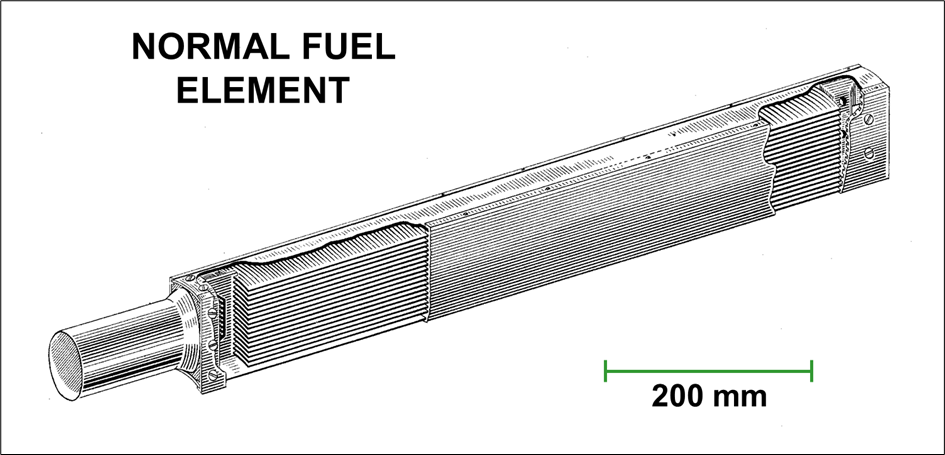
\includegraphics[width=0.75\linewidth]{img/PS_RA2.png}
    \caption{Palivový soubor reaktoru RA-2}
    \label{fig:enter-label}
\end{figure}

\subsubsection*{Důsledky nehody}

Operátor, který byl v té době jedinou osobou přítomnou v reaktorové hale, obdržel smrtelnou dávku radiace odhadovanou na 20-21 Gy a 17-22 Gy od neutronů. Nejvyšší expozice byla zaznamenána v horní pravé části jeho těla. Asi 25 minut po nehodě se u něj objevily příznaky akutní radiační nemoci, jako zvracení, silné bolesti hlavy a průjem. Jeho stav se rychle zhoršoval a zemřel dva dny po nehodě, 25. září 1983.

Další dvě osoby, které se nacházely v kontrolní místnosti, obdržely dávky přibližně 0.15 a 0.2 od gama. 11 dalších pracovníků bylo vystaveno dávkám ??? bez zjevných zdravotních následků.

\subsubsection*{Vyšetřování a poučení}

Vyšetřování odhalilo několik závažných porušení bezpečnostních protokolů:

\begin{itemize}
    \item \textbf{Nedostatečné odstranění moderátoru:} Moderující voda nebyla před úpravami konfigurace AZ zcela odstraněna.
    \item \textbf{Nesprávné umístění palivových článků:} Dva palivové články byly ponechány uvnitř reaktoru v kontaktu s grafitovým reflektorem.
    \item \textbf{Chybné pořadí operací:} Sekvence změn v pozicích palivových článků snížila podkritičnost systému.
    \item \textbf{Nesprávné vložení palivových článků:} Dva články byly vloženy bez odpovídajících kadmiových regulačních desek.
    \item \textbf{Nedostatečný dohled:} Operace byly prováděny bez přítomnosti bezpečnostního pracovníka nebo supervizora. Neexistence schváleného plánu pro změnu konfigurace
\end{itemize}

Tato nehoda, klasifikovaná jako úroveň 4 na Mezinárodní stupnici jaderných událostí (INES), zdůrazňuje kritickou důležitost přísného dodržování bezpečnostních protokolů, školení personálu a důsledného dohledu při provozu jaderných zařízení.


